%%%%%%%%%%%%%%%%%%%%%%%%%%%%%%%%%%%%%%%%%%%%%%%%%%%%%%%%%%%%%%%%%%% 
%                                                                 %
%                            CHAPTER                              %
%                                                                 %
%%%%%%%%%%%%%%%%%%%%%%%%%%%%%%%%%%%%%%%%%%%%%%%%%%%%%%%%%%%%%%%%%%% 

\chapter{Accelerating the software implementation using HLS}
\label{ch:HardwareImpl}

\section{Analysing software performance}

In the SDSoC environment, it is possible to analyze the software running on the SoC chip using a TCF profiler. After running this analysis, the TCF profiler returns an overview of the functions, sorted on the amount of time spent when running. The analysis is shown in figure \ref{fig:softwareFunctionUsage}

\begin{figure}[H]
	\centering
	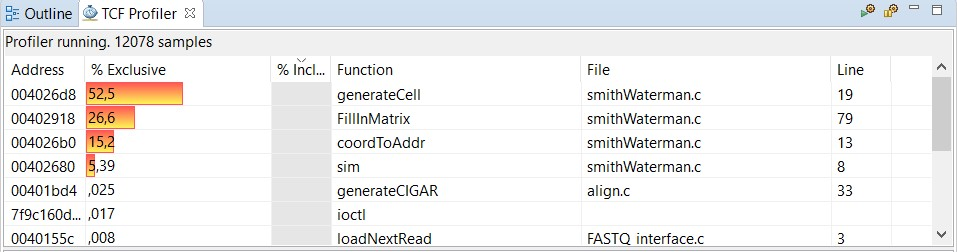
\includegraphics[width=0.75\textwidth]{speedup/softwareFunctionUsage.jpg}
	\caption{a TCF profile of the software implementation}
	\label{fig:softwareFunctionUsage}
\end{figure}

When examining this analysis, we should keep in mind that the generateCell, coordToAddr, and sim functions are inline functions used in the FillInMatrix method. Just as suspected the software spends almost all of its time in these methods, so it's worth it to try to accelerate these functions.

\section{Recoding parts of the software to be more hardware friendly}

\subsection{Recoding the Cell generation layer}

Back in 2011, Vermij E. did a thesis\cite{Vermij} on RVE (recursive variable expansion). He discusses the most efficient ways to program a processing element to generate one value in the alignment matrix. His results can be found in figure \ref{fig:PE}. 

\begin{figure}[H]
	%src=file:///D:/Erasmus/thesis/interessante%20papers/masterthesis%20Smith-Waterman%20op%20FPGA%20(TU%20Delft).pdf
	\centering
	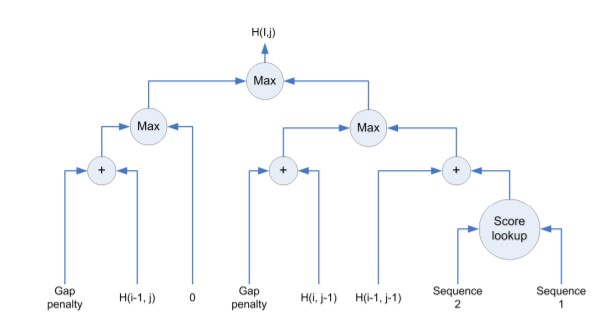
\includegraphics[width=0.75\textwidth]{speedup/PE.jpg}
	\caption{The optimal processing found in the thesis from Vermij E.\cite{Vermij}}
	\label{fig:PE}
\end{figure}

It seemed like a good idea to reimplement the generatecell function, using this newly found scheme. However, it is also important to keep track of where the value comes from. Therefore, the following (new) code was adopted for generating a cell:

\begin{lcverbatim}
//calculate the possible  values
CELL diagonalCELL = { diagonal.value + sim(refVal, seqVal), 1 };
CELL leftCELL = { left.value - gp, 2 };
CELL upCELL = { up.value - gp, 3 };
CELL zeroCELL = { 0, 0 };

CELL upstreamA = (leftCELL.value > upCELL.value) ? leftCELL : upCELL;
CELL upstreamB = (diagonalCELL.value > zeroCELL.value) ? 
diagonalCELL : zeroCELL;

CELL newCell = (upstreamA.value > upstreamB.value) ? upstreamA : upstreamB;

//Return the cell:
return newCell;
\end{lcverbatim}

Where the second attribute in the CELL type is the direction.

\subsection{Recoding the FillIn layer}

HLS does not support input and output from the same memory locations in hardware, therefore, the Fillin layer also has to be recoded. We will take a look at the data dependencies again:

\begin{figure}[H]
	\centering
	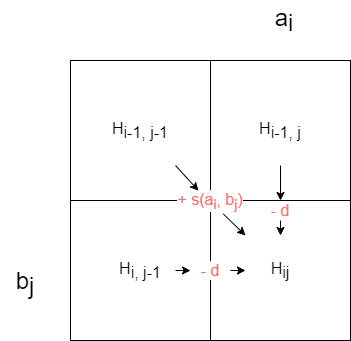
\includegraphics[width=0.3\textwidth]{ExisMethods/Dependencies_SW.png}
	\caption{Data dependencies for generating a cell in the alignment matrix}
	\label{fig:DatDep2}
\end{figure}

Since the current cell only depends on the left-up 3 cells, we can compute every cell on the diagonal in parallel. Therefore, 3 arrays where created: one contains the current diagonal being generated, one contains the previous diagonal for the cell above and the cell to the left of the current generated cell, and one for the diagonal before that. This last array will house the left-up cell also needed for the new cell generation. A schematic of the data structures used can be found in table \ref{tbl:arraytable}

\begin{table}[H]
	\centering
	\begin{tabular}{|l|lllllllllll|l|l|l|}
		\cline{1-10} \cline{13-15}
		\multicolumn{1}{|c|}{\textbf{}} & \multicolumn{1}{r|}{\textbf{ref}} & \multicolumn{1}{l|}{\textbf{T}} & \multicolumn{1}{l|}{\textbf{G}} & \multicolumn{1}{l|}{\textbf{T}} & \multicolumn{1}{l|}{\textbf{T}} & \multicolumn{1}{l|}{\textbf{A}} & \multicolumn{1}{l|}{\textbf{C}} & \multicolumn{1}{l|}{\textbf{G}} & \multicolumn{1}{l|}{\textbf{G}} & \textbf{}       & \textbf{} & \textbf{ppD}              & \textbf{pD}               & \textbf{cD}               \\ \cline{1-10} \cline{13-15} 
		\textbf{seq}                    & 0                                 & 0                               & 0                               & 0                               & 0                               & \cellcolor[HTML]{9AFF99}0       & \cellcolor[HTML]{96FFFB}0       & \cellcolor[HTML]{FFCCC9}0       & 0                               &                 &           & \cellcolor[HTML]{9AFF99}0 & \cellcolor[HTML]{96FFFB}0 & \cellcolor[HTML]{FFCCC9}0 \\ \cline{1-1} \cline{13-15} 
		\textbf{G}                      & 0                                 & 0                               & 3                               & 1                               & \cellcolor[HTML]{9AFF99}0       & \cellcolor[HTML]{96FFFB}0       & \cellcolor[HTML]{FFCCC9}?       &                                 &                                 &                 &           & \cellcolor[HTML]{9AFF99}0 & \cellcolor[HTML]{96FFFB}0 & \cellcolor[HTML]{FFCCC9}? \\ \cline{1-1} \cline{13-15} 
		\textbf{G}                      & 0                                 & 0                               & 3                               & \cellcolor[HTML]{9AFF99}1       & \cellcolor[HTML]{96FFFB}0       & \cellcolor[HTML]{FFCCC9}?       &                                 &                                 &                                 & =\textgreater{} &           & \cellcolor[HTML]{9AFF99}1 & \cellcolor[HTML]{96FFFB}0 & \cellcolor[HTML]{FFCCC9}? \\ \cline{1-1} \cline{13-15} 
		\textbf{T}                      & 0                                 & 3                               & \cellcolor[HTML]{9AFF99}1       & \cellcolor[HTML]{96FFFB}6       & \cellcolor[HTML]{FFCCC9}?       &                                 &                                 &                                 &                                 &                 &           & \cellcolor[HTML]{9AFF99}1 & \cellcolor[HTML]{96FFFB}6 & \cellcolor[HTML]{FFCCC9}? \\ \cline{1-1} \cline{13-15} 
		\textbf{T}                      & 0                                 & \cellcolor[HTML]{9AFF99}3       & \cellcolor[HTML]{96FFFB}1       & \cellcolor[HTML]{FFCCC9}?       &                                 &                                 &                                 &                                 &                                 &                 &           & \cellcolor[HTML]{9AFF99}3 & \cellcolor[HTML]{96FFFB}1 & \cellcolor[HTML]{FFCCC9}? \\ \cline{1-1} \cline{13-15} 
		\textbf{G}                      & \cellcolor[HTML]{9AFF99}0         & \cellcolor[HTML]{96FFFB}1       & \cellcolor[HTML]{FFCCC9}?       &                                 &                                 &                                 &                                 &                                 &                                 &                 &           & \cellcolor[HTML]{9AFF99}0 & \cellcolor[HTML]{96FFFB}1 & \cellcolor[HTML]{FFCCC9}? \\ \cline{1-1} \cline{13-15} 
	\end{tabular}
	\caption{The 3 newly created arrays to house the data needed for generating the next diagonal of cells. The '?' in the cD array (red) is represents cells that are currently being generated. Notice that all the information needed to generate the new cell is present in the other 2 arrays}
	\label{tbl:arraytable}
\end{table}

Also keep note that the FillIn layer should also keep track of the maximum location in the matrix. Having gained this new information, we can recode the FillInlayer as follows:

\begin{enumerate}
	\item Create the arrays $ppD$, $pD$ and $cD$. They should be the length of the sequence. All are initialized on zeros.
	\item Start the current diagonal at the second column.
	\item \label{everyCell}For every cell at the diagonal, do the following:
	\begin{enumerate}
		\item Check for edge cases. The row has to be smaller than the length of the sequence, the column can't be 0 or smaller and the column can't be bigger than the length of the reference.
		\item Generate the new cell using the data in the $ppD$ and $pD$ arrays.
		\item Write this new cell to memory, and its value to the cD array.
		\item Check if it is bigger than the current maximum. If so, the current maximum should be this new cell. 
	\end{enumerate}
	\item Set current diagonal to the next one.
	\item Shift the values ($cD \rightarrow pD$ and $pD \rightarrow ppD$) and repeat from step \ref{everyCell}, until the full matrix is filled.
	\item Return the position of the maximum to the alignment level.
\end{enumerate}

\section{Hardware acceleration}

\subsection{Acceleration}
//TODO bespreek pragmas used and speedup

- Bitwidth of (packed) data on axi master must be power of 2. => change the int to int16\_t and direction to uint16\_t (really wastefull towards memory) but no other choice without major remodel. (maybe do if enough time)

\subsection{Comparison with the software}

//TODO